\newcommand*{\TeXturedVERSION}{1.5.0} %% TeXtured 2025-08-06
%%%%%%%%%%%%%%%%%%%%%%%%%%%%%%%%%%%%%%%%%%%%%%%%%%%%%%%%%%%%%%%%%%%%%%%
%% NOTE: If you find any issues or have any suggestions, please open %%
%%       an Issue on GitHub: https://github.com/jdujava/TeXtured     %%
%%%%%%%%%%%%%%%%%%%%%%%%%%%%%%%%%%%%%%%%%%%%%%%%%%%%%%%%%%%%%%%%%%%%%%%

%% Enable built-in LaTeX support for PDF/A compliance (must be before `\documentclass`)
\DocumentMetadata{lang=fr, pdfversion=1.7, pdfstandard=A-2u}
\input{preamble/pdfA-compliance/glyphtounicode}

%% NOTE: Choose the desirable page layout version (electronic vs print)
\documentclass[12pt,a4paper]{report}                      % single-side (electronic)
% \documentclass[12pt,a4paper,openright,twoside]{report}  % two-sided (for printing)

%% Set some toggle flags to control some of the document properties
\input{preamble/toggles}
% \FANCYfalse % disable some of the more fancy stylistic choices
%% NOTE: Comment out the following lines for the final version
\WIPtrue            % THIS IS A WORK-IN-PROGRESS VERSION
% \EXTRAMARGINtrue  % add extra right margin in WIP version (for notes/corrections)
% \LINKBOXESfalse   % disable reference/link boxes for faster compilations
\CENSORtrue         % THIS IS A CENSORED VERSION

%% Preamble - data, packages, macros, and more
\def\IVEVO{1}
\def\EVODraft{Brouillon}
\def\EVOTitle{Manuel d’utilisation IV-Evo}
\def\EVOProduct{IV-Evo pour Golf/Jetta II}
\input{preamble/main}

%% Only uncommented files are included (faster compilation)
%% NOTE: If no files are uncommented, all files are included
\emergencystretch=2em
\begin{document}
\selectlanguage{french}

\frontmatter
\include{frontmatter_fr/title}
% \include{frontmatter/declaration}
% \include{frontmatter/dedication}
% \include{frontmatter/information}

\contentsandlists

\mainmatter
\chapter{Sécurité et alimentation}
Ne jamais alimenter IV-Evo simultanément par USB et par l'entrée KL30. Avant de brancher USB, déconnecter complètement l'indicateur du faisceau du véhicule et de toute alimentation externe. Ne pas brancher USB lorsque l'indicateur est installé et câblé dans la voiture. La documentation fournie exclut la garantie et les retours pour cette utilisation interdite.

Couper l'alimentation avant de modifier le câblage. Vérifier les numéros de broches et le schéma correspondant. Au soleil, la face avant peut dépasser 90 $^\circ$C même lorsque l'appareil est éteint ; la laisser refroidir avant de la toucher. Effectuer la configuration véhicule à l'arrêt.

\chapter{Présentation et contenu du colis}
IV-Evo est un indicateur PHOL-LABS Kft doté d'un ESP32-C3, d'un écran IPS de 160\,\texttimes\,80 pixels et d'une face avant en verre trempé. Ce manuel concerne la version Golf/Jetta II. La source mentionne aussi des variantes Golf, Jetta, Polo, Audi et LADA ; vérifier la variante mécanique avant installation.

Il prend en charge Wi-Fi, Bluetooth LE, les applications et scripts de capteurs Lua, les images JPG/PNG/BMP et des animations simples 2D et 3D. L'application gère l'affichage et les interactions ; le script du capteur fournit les mesures. Application, capteur et étalonnage doivent correspondre.

La liste du colis comprend un indicateur de type bouton et une prise KF2510 avec fils. Les capteurs, contrôleurs externes et Digifiz Next ne figurent pas dans cette liste. Un passage commercial mentionne un programmateur, mais la liste explicite ne l'inclut pas.

\chapter{Configuration Wi-Fi}
Le Wi-Fi est désactivé en fonctionnement normal. Pendant la configuration, placer le téléphone à environ 10–20 cm de l'indicateur. Le mot de passe par défaut est 1234567890 et le panneau est accessible à http://192.168.4.1.

USB étant débranché, mettre le contact ou l'alimentation puis appuyer immédiatement sur le bouton arrière. Un code QR apparaît. Désactiver les données mobiles, scanner le code et connecter le téléphone au réseau Wi-Fi de l'indicateur. Ouvrir le panneau dans le navigateur, choisir l'application et le capteur adapté, enregistrer puis couper et remettre le contact.

En cas d'échec, rapprocher le téléphone et vérifier qu'il reste connecté au réseau de l'indicateur malgré l'absence d'Internet. Répéter si nécessaire le démarrage en mode QR. Le bouton arrière permet aussi d'interagir avec les applications et de choisir le mode de démarrage lors de la programmation initiale.

USB est prévu pour la programmation initiale ; l'interface web est recommandée pour les mises à jour suivantes. Déconnecter tous les fils du véhicule avant d'utiliser USB. Suivre les instructions du micrologiciel concerné ; la source ne décrit ni procédure de récupération ni menu de téléversement.

\begin{figure}[H]
\centering
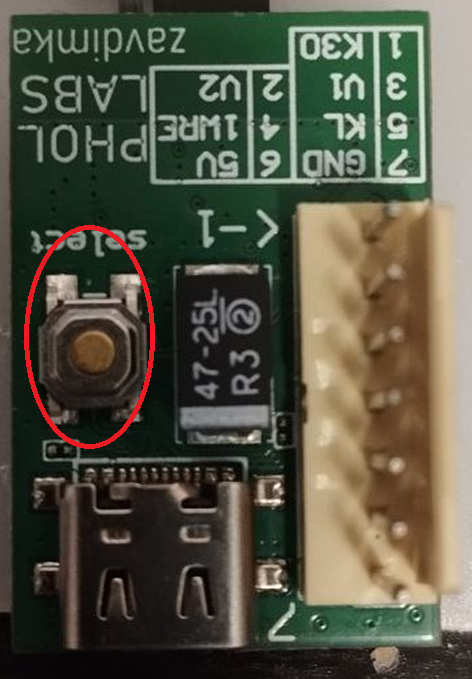
\includegraphics[width=.85\textwidth,height=.60\textheight,keepaspectratio]{figures/ivevo/image11.png}
\caption{Configuration Wi-Fi}
\end{figure}

\chapter{Connecteur et schémas}
Le connecteur KF2510 à sept broches est numéroté sur la carte. Utiliser l'orientation de la photographie et les numéros, pas seulement les couleurs des fils. Broche 1 : K30/KL30, alimentation ; 2 : V2 ; 3 : V1 ; 4 : 1WRE, One-Wire ; 5 : KL, K-Line réservée ; 6 : sortie +5 V, 30 mA maximum ; 7 : GND, masse.

Le schéma du voltmètre précise la K-Line réservée et la limite de courant de la sortie +5 V. Les limites générales de tension des entrées analogiques ne sont pas indiquées. Les 12 V mentionnés pour Check Engine ne constituent pas une spécification des autres entrées. Utiliser le schéma adapté au capteur.

Les illustrations originales conservent leurs annotations anglaises ; les fonctions correspondantes sont expliquées dans ce manuel.

\begin{figure}[H]
\centering
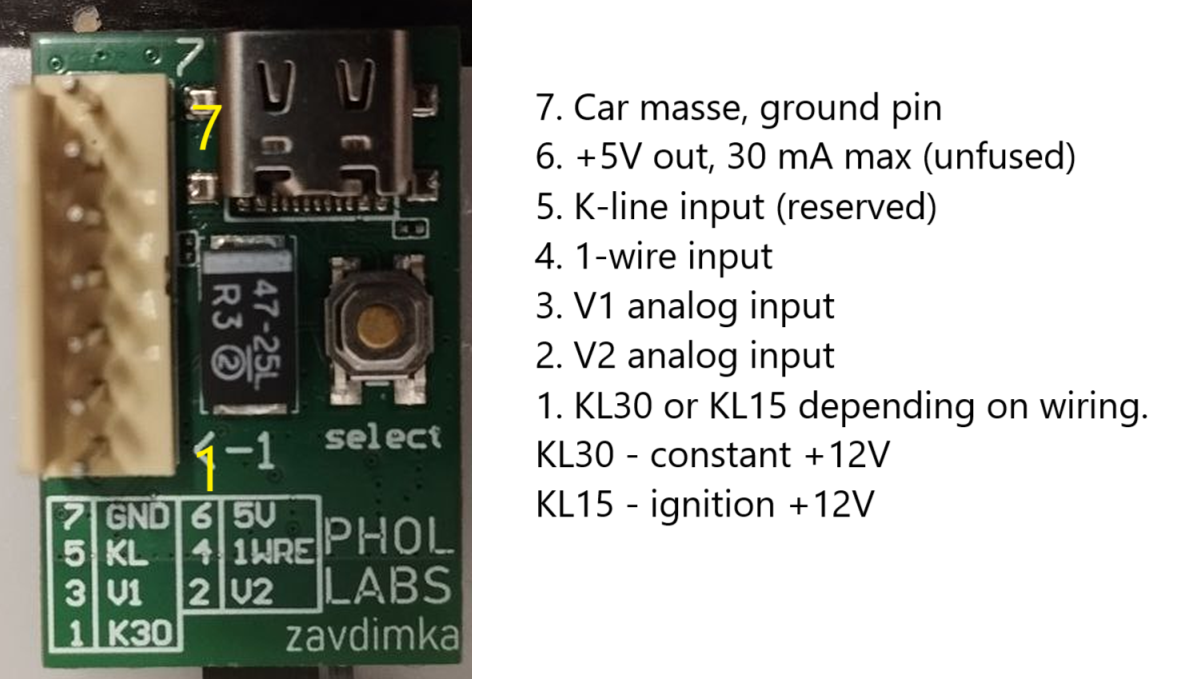
\includegraphics[width=.85\textwidth,height=.60\textheight,keepaspectratio]{figures/ivevo/image20.png}
\caption{Connecteur et schémas}
\end{figure}
\clearpage
\section{Voltmètre}

\begin{figure}[H]
\centering
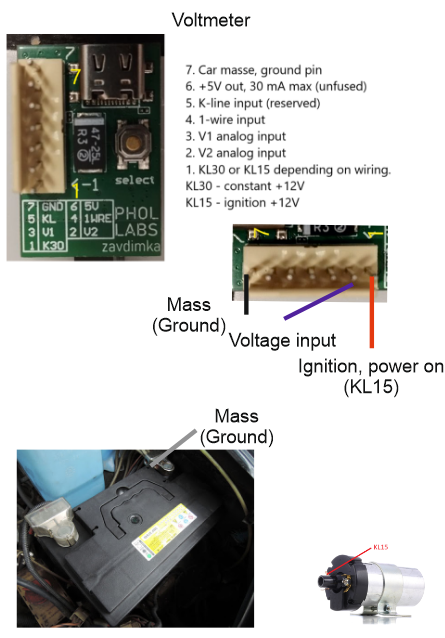
\includegraphics[width=.85\textwidth,height=.60\textheight,keepaspectratio]{figures/ivevo/image5.png}
\caption{Voltmètre}
\end{figure}
\clearpage
\section{Indicateur de rapport}

\begin{figure}[H]
\centering
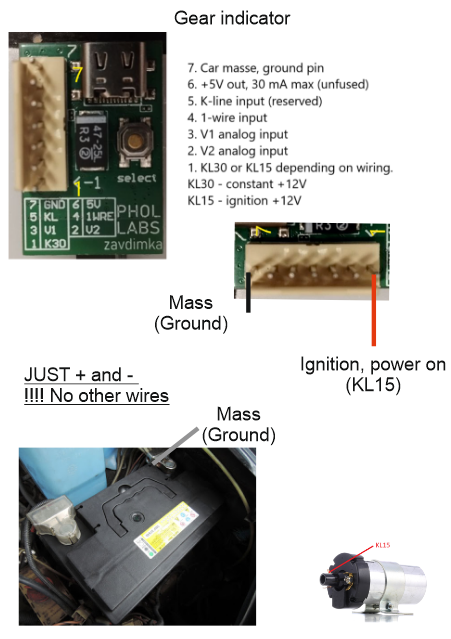
\includegraphics[width=.85\textwidth,height=.60\textheight,keepaspectratio]{figures/ivevo/image6.png}
\caption{Indicateur de rapport}
\end{figure}
\clearpage
\section{Pression d’huile}

\begin{figure}[H]
\centering
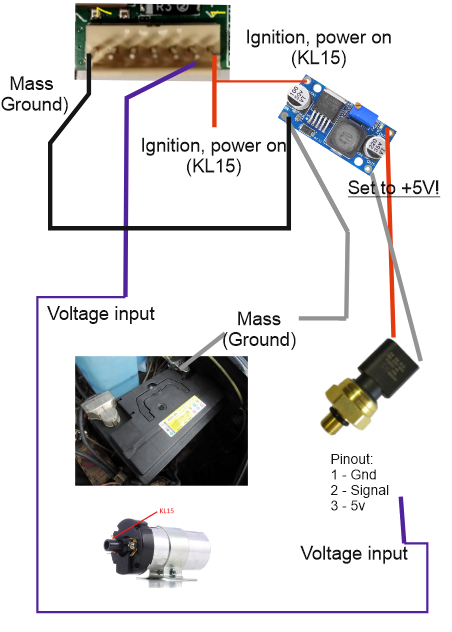
\includegraphics[width=.85\textwidth,height=.60\textheight,keepaspectratio]{figures/ivevo/image1.png}
\caption{Pression d’huile}
\end{figure}
\clearpage
\section{Thermomètre NTC}

\begin{figure}[H]
\centering
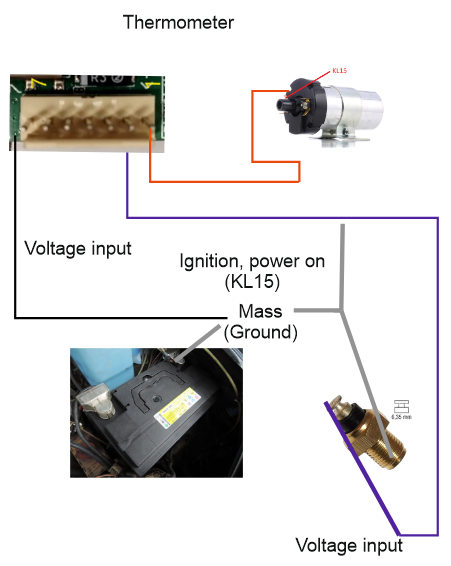
\includegraphics[width=.85\textwidth,height=.60\textheight,keepaspectratio]{figures/ivevo/image13.png}
\caption{Thermomètre NTC}
\end{figure}
\clearpage
\section{Thermomètre numérique}

\begin{figure}[H]
\centering
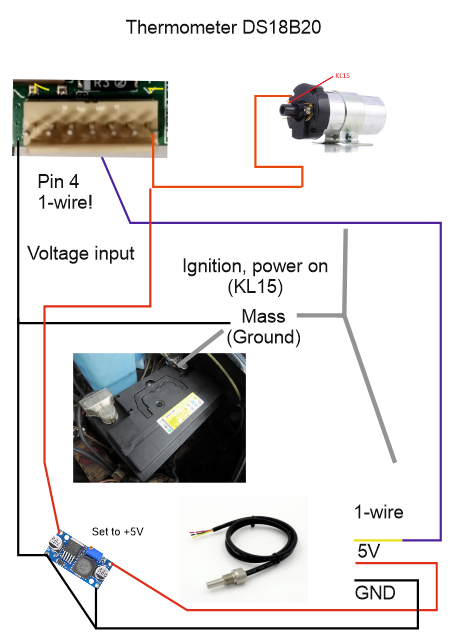
\includegraphics[width=.85\textwidth,height=.60\textheight,keepaspectratio]{figures/ivevo/image8.png}
\caption{Thermomètre numérique}
\end{figure}
\clearpage
\section{Lambda large bande}

\begin{figure}[H]
\centering
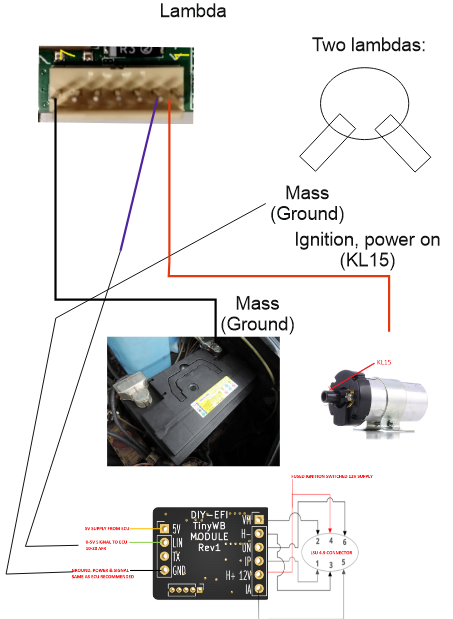
\includegraphics[width=.85\textwidth,height=.60\textheight,keepaspectratio]{figures/ivevo/image3.png}
\caption{Lambda large bande}
\end{figure}
\clearpage
\section{Suralimentation}

\begin{figure}[H]
\centering
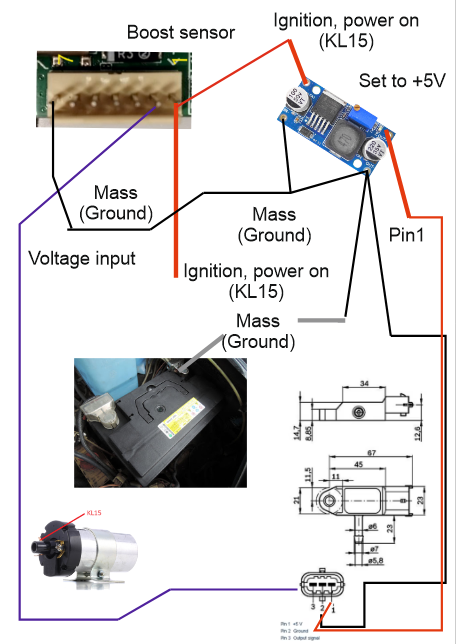
\includegraphics[width=.85\textwidth,height=.60\textheight,keepaspectratio]{figures/ivevo/image17.png}
\caption{Suralimentation}
\end{figure}

\chapter{Applications et étalonnage}
\section{Voltmètre}
Affiche la tension de la batterie en fonctionnement. evo\_v\_l présente une valeur numérique avec une icône de batterie ; iv\_evo\_v\_t utilise un affichage à segments semblable à IV-Nano.

\begin{figure}[H]
\centering
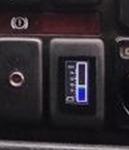
\includegraphics[width=.85\textwidth,height=.60\textheight,keepaspectratio]{figures/ivevo/image16.png}
\caption{Voltmètre}
\end{figure}

\begin{figure}[H]
\centering
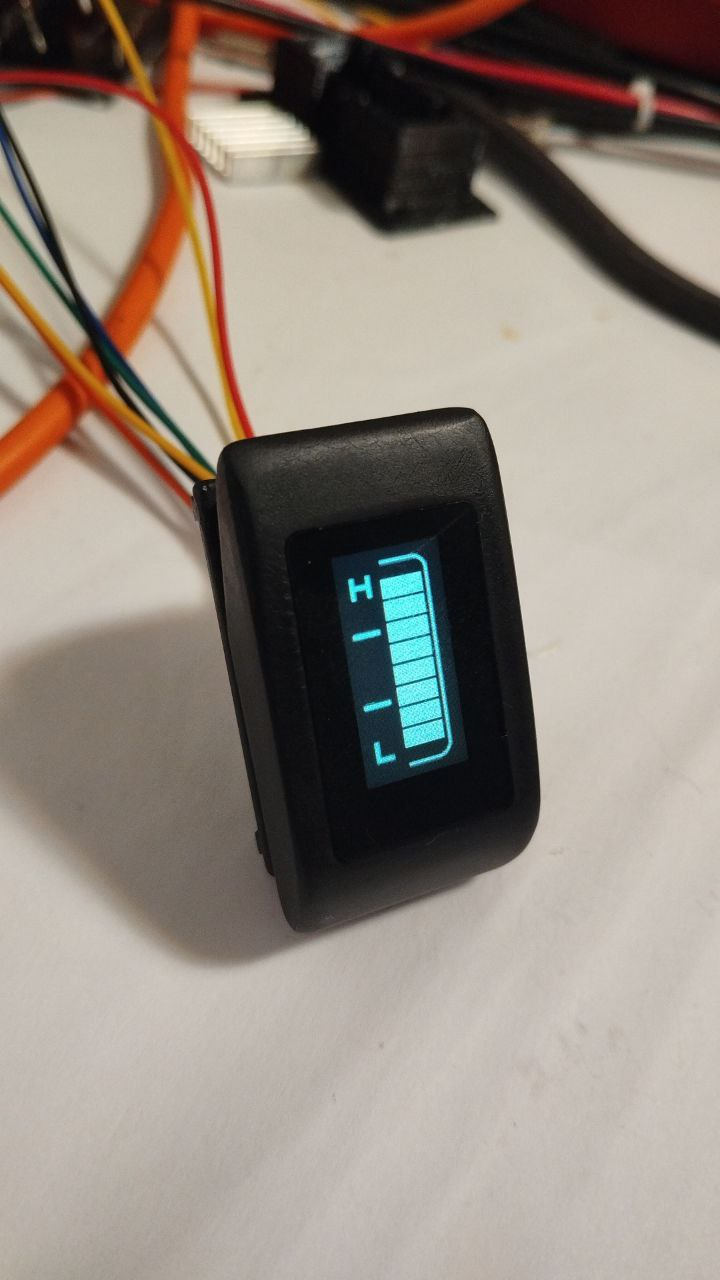
\includegraphics[width=.85\textwidth,height=.60\textheight,keepaspectratio]{figures/ivevo/image15.png}
\caption{Voltmètre}
\end{figure}

\begin{figure}[H]
\centering
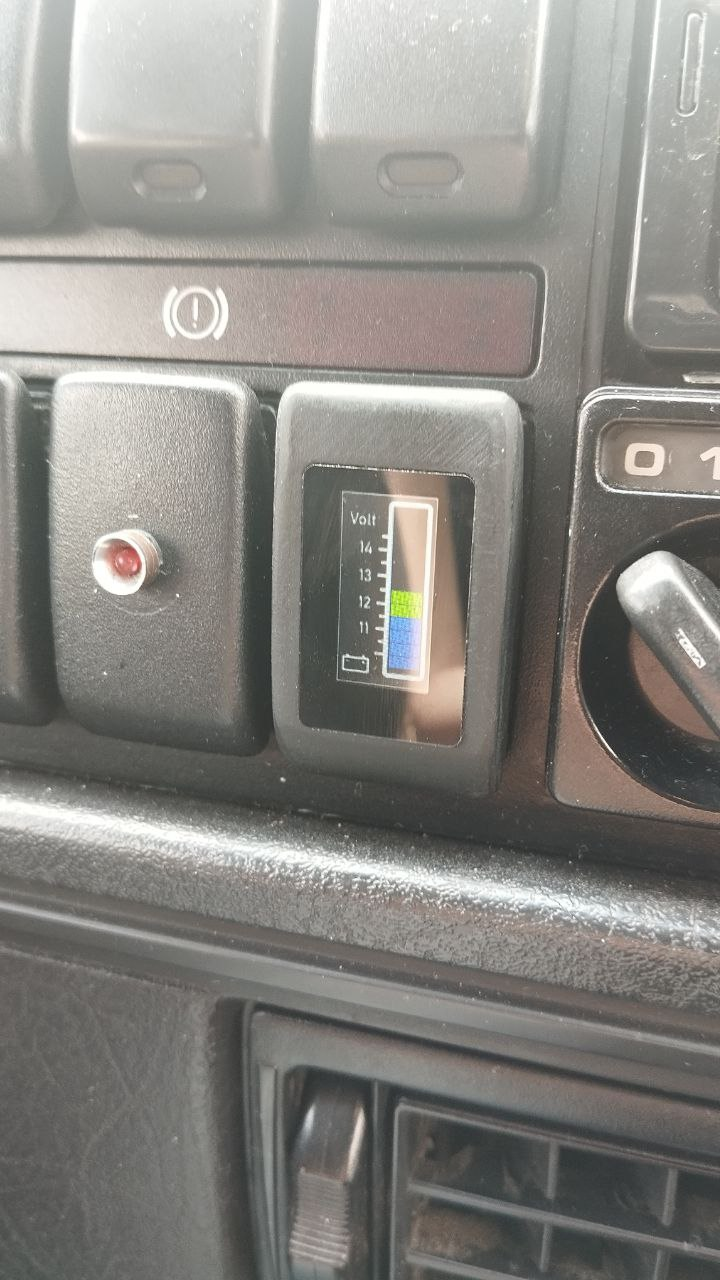
\includegraphics[width=.85\textwidth,height=.60\textheight,keepaspectratio]{figures/ivevo/image2.png}
\caption{Voltmètre}
\end{figure}
\section{Pression d'huile (Barometer)}
Un capteur est obligatoire ; le modèle prévu est VAG 03C906051A. Malgré la sortie +5 V interne, la source recommande un convertisseur DC/DC externe pour le capteur. Suivre le schéma de pression d'huile et utiliser un étalonnage adapté au capteur.

\begin{figure}[H]
\centering
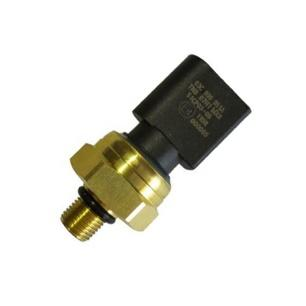
\includegraphics[width=.85\textwidth,height=.60\textheight,keepaspectratio]{figures/ivevo/image21.jpg}
\caption{Pression d'huile (Barometer)}
\end{figure}
\section{Température (Thermo)}
Choisir un capteur NTC ou un DS18B20 numérique et le script correspondant. Les sondes DS18B20 câblées sont acceptées. Pour le NTC, Ossca 01176 ou un capteur Golf 2 compatible est recommandé. Sur le capteur Ossca, relier les broches du capteur 1 et 2 ; la résistance NTC est raccordée à la broche du capteur 3. Ce sont les numéros du capteur, pas les broches d'alimentation de l'indicateur.

\begin{figure}[H]
\centering
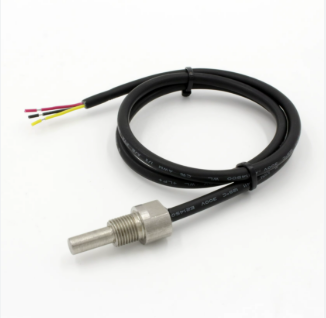
\includegraphics[width=.85\textwidth,height=.60\textheight,keepaspectratio]{figures/ivevo/image14.png}
\caption{Température (Thermo)}
\end{figure}

\begin{figure}[H]
\centering
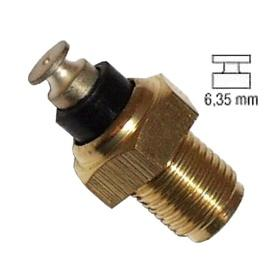
\includegraphics[width=.85\textwidth,height=.60\textheight,keepaspectratio]{figures/ivevo/image19.jpg}
\caption{Température (Thermo)}
\end{figure}
\section{Indicateur de rapport}
Affiche R et les rapports 1–5. Il calcule le rapport à partir de la vitesse et du régime reçus de Digifiz Next par Bluetooth LE. La marche arrière nécessite un signal positif sur une entrée conformément au schéma. Digifiz Next doit disposer du micrologiciel 1.0.14 ou ultérieur.

Pour cette application, raccorder la broche 1 (K30/KL30) au +12 V KL15 après contact et la broche 7 à la masse. Au démarrage, un tiret signifie qu'aucun rapport n'est sélectionné ; l'appareil recherche Digifiz Next. En mode QR, choisir l'application iv\_gear et le capteur volts1, enregistrer et remettre le contact.

Dans le panneau web Digifiz Next, étalonner la vitesse avec le GPS, le régime et la table des rapports selon le véhicule. La source suggère 80–100 km/h comme référence : uniquement dans des conditions légales et sûres, avec un passager notant les valeurs. Les valeurs de régime 1500, 3000 et 400 n'ont ni unité ni correspondance moteur clairement définies. Consulter les instructions du combiné pour le moteur concerné sans deviner les réglages.

\begin{figure}[H]
\centering
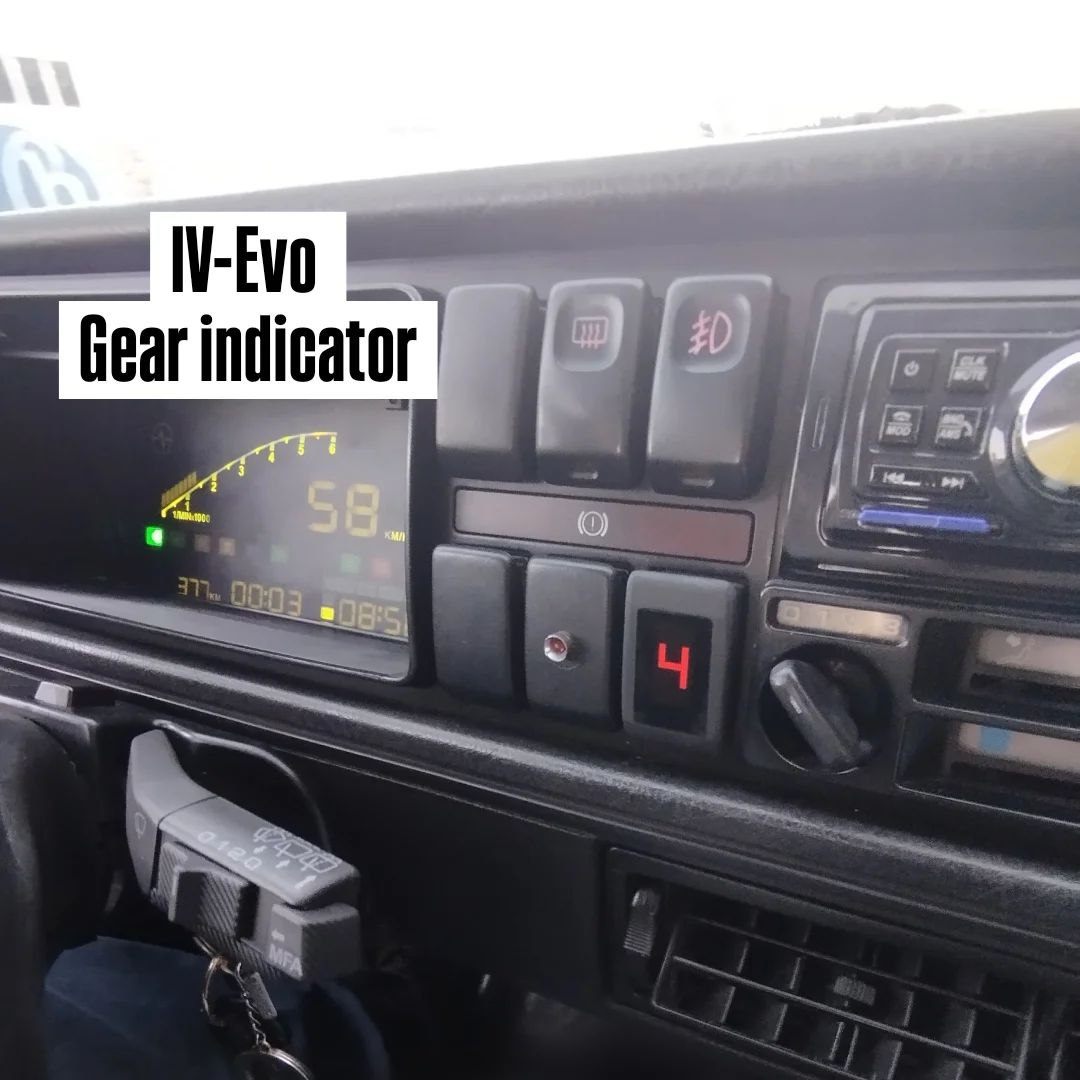
\includegraphics[width=.85\textwidth,height=.60\textheight,keepaspectratio]{figures/ivevo/image18.png}
\caption{Indicateur de rapport}
\end{figure}

\begin{figure}[H]
\centering
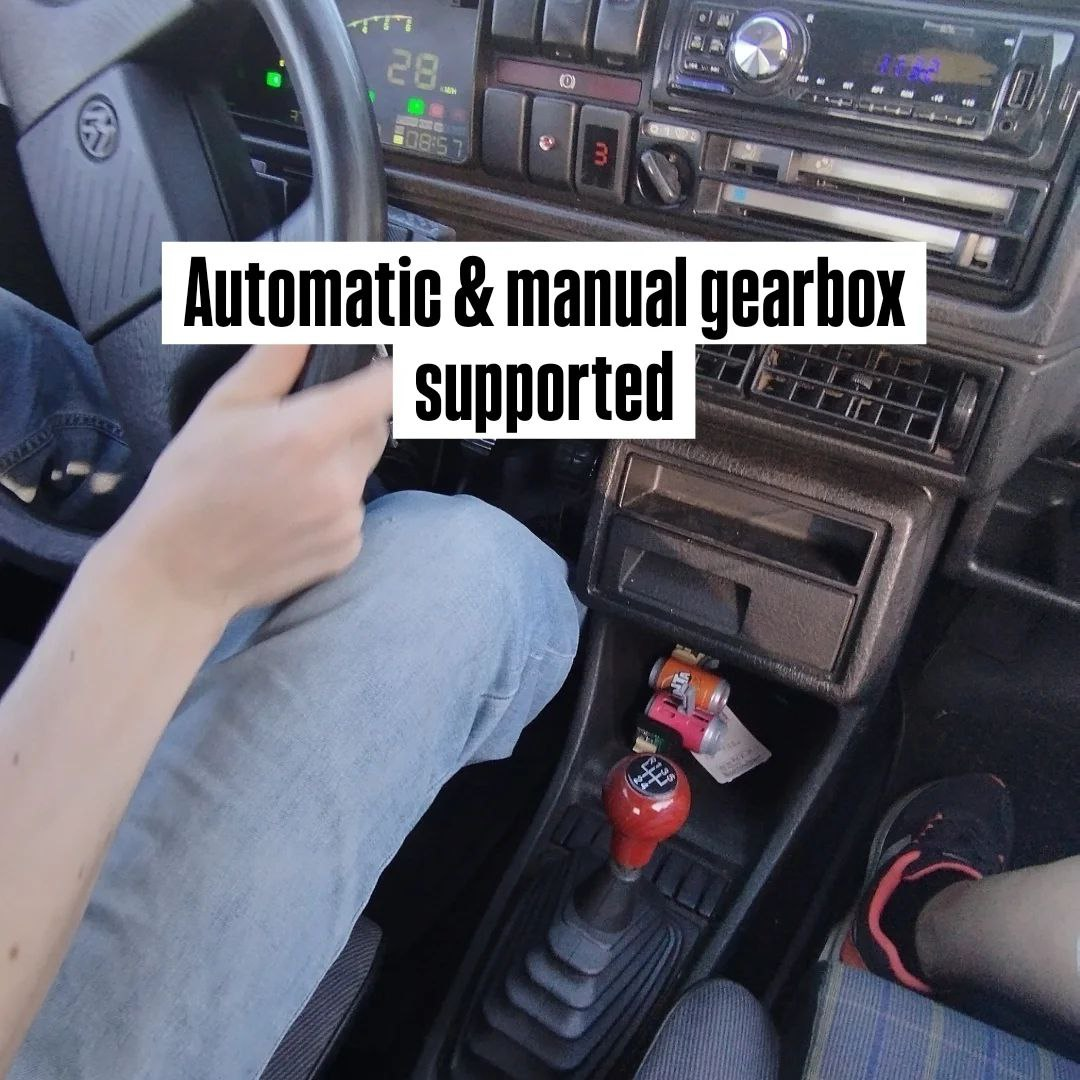
\includegraphics[width=.85\textwidth,height=.60\textheight,keepaspectratio]{figures/ivevo/image10.png}
\caption{Indicateur de rapport}
\end{figure}
\section{Lambda}
Ne pas raccorder l'indicateur à la sonde lambda d'origine du Golf 2. La source exige une sonde de mesure séparée ; si la sonde d'origine est conservée, deux sondes sont installées. Une sonde à bande étroite produit environ 0,1 V (pauvre) à 0,9 V (riche), sans mesure précise du rapport air-carburant. Le raccordement direct nécessite un étalonnage.

Une sonde large bande nécessite son propre contrôleur ; IV-Evo ne peut pas la piloter directement. La Bosch LSU 4.9 est recommandée avec un contrôleur compatible, par exemple SLC Free, DIY-EFI TinyWB, Sigma Lambda Controller Free 2 ou rusEFI wideband. Raccorder la sonde suivant les instructions du contrôleur et utiliser sa sortie analogique. Elle peut être de 0–5 V, 0,5–4,5 V ou 0–1 V ; conversion et courbe d'étalonnage doivent correspondre.

\begin{figure}[H]
\centering
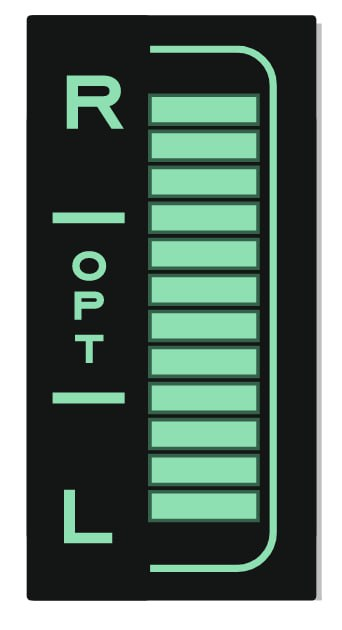
\includegraphics[width=.85\textwidth,height=.60\textheight,keepaspectratio]{figures/ivevo/image7.png}
\caption{Lambda}
\end{figure}
\section{Check Engine}
Affiche « Check Engine » lorsque la broche 2 (V2) reçoit 12 V et laisse l'écran vide à 0 V. Il s'agit d'un indicateur de signal ; aucune lecture de codes défaut ni interface OBD n'est décrite.

\begin{figure}[H]
\centering
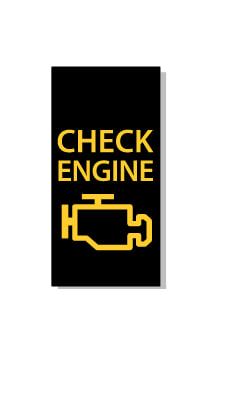
\includegraphics[width=.85\textwidth,height=.60\textheight,keepaspectratio]{figures/ivevo/image4.png}
\caption{Check Engine}
\end{figure}
\section{Pression de suralimentation (Boost)}
La source indique un capteur à trois broches, alimenté en +5 V, avec un trou de fixation et une plage de 20–250 kPa. La tension nominale de sortie est +1,8 V. La pression correspondante et la fonction de transfert complète ne sont pas fournies. Confirmer le capteur exact et sa courbe avant étalonnage ; ne pas déduire une pente d'un seul point.

\begin{figure}[H]
\centering
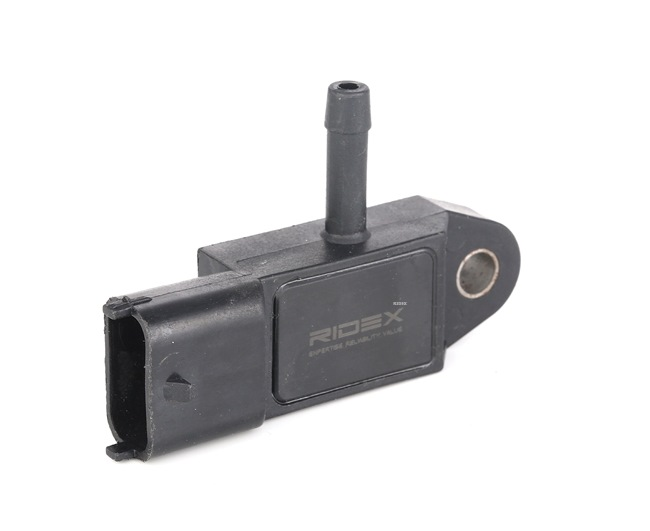
\includegraphics[width=.85\textwidth,height=.60\textheight,keepaspectratio]{figures/ivevo/image9.png}
\caption{Pression de suralimentation (Boost)}
\end{figure}
\section{Horloge}
L'application d'exemple utilise l'horloge système. L'heure n'est pas conservée au redémarrage ; sans nouveau réglage, elle sert de compteur de durée du trajet.

\begin{figure}[H]
\centering
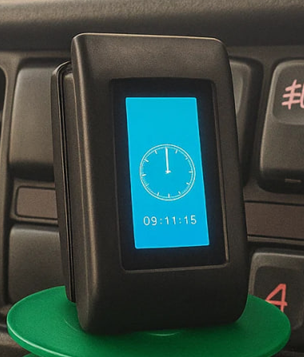
\includegraphics[width=.85\textwidth,height=.60\textheight,keepaspectratio]{figures/ivevo/image12.png}
\caption{Horloge}
\end{figure}
\section{Limites de la documentation}
Les tolérances générales d'alimentation, les températures de fonctionnement et l'indice de protection du boîtier ne sont pas fournis. Ne pas appliquer les spécifications Nano à IV-Evo.

\appendix
\chapter{Référence de l'API Lua}
\section{Modèle d'exécution}
app.lua renvoie une table M. M.loop() est obligatoire et s'exécute de façon répétée ; M.init(), M.event(event\_type) et M.cleanup() sont facultatifs. Sans loop, l'application est rejetée. En cas d'erreur d'exécution, le micrologiciel peut basculer vers une application de secours.

Le script dans sensor/*.lua renvoie une table sensor avec sensor.get(index), qui renvoie une valeur numérique. Le micrologiciel expose sensor globalement. apppath est le chemin du dossier de l'application courante. Charger les modules avec require("module") ; pcall(require, "module") convient aux modules facultatifs.
\section{Ressources et affichage}
loadimg et loadfont renvoient un identifiant ou nil ; free libère les images et polices chargées. fill remplit l'écran entier. update transmet l'image puis efface l'écran en noir. drawpolygon demande un nombre pair de coordonnées, au moins quatre éléments. Appeler update une fois par image et libérer les ressources dans cleanup.
\section{Autres modules}
system contrôle délai, rétroéclairage, résistance de tirage V2, sortie 5 V et veille, et lit boutons, ADC et heure. onewire recherche les DS18B20 et lit leur température en Celsius. nvs utilise l'espace NVS app ; get renvoie une chaîne ou nil et push un booléen. ble initialise BLE et fournit régime, vitesse et rapport.
\section{display}
\begin{itemize}
\item display.loadimg(path) -> img\_handle|nil
\item display.loadfont(path) -> font\_handle|nil
\item display.free(handle)
\item display.fill(color)
\item display.update()
\item display.drawimg(img, x, y)
\item display.string(font, x, y, text, color)
\item display.fillrect(x, y, width, height, color)
\item display.drawline(x1, y1, x2, y2, color)
\item display.drawcircle(x, y, r, color)
\item display.drawfillcircle(x, y, r, color)
\item display.drawroundrect(x1, y1, x2, y2, r, color)
\item display.drawarrow(x0, y0, x1, y1, w, color)
\item display.drawfillarrow(x0, y0, x1, y1, w, color)
\item display.drawpolygon(\{x1, y1, x2, y2, ...\}, color)
\item display.RED
\item display.GREEN
\item display.BLUE
\item display.WHITE
\item display.BLACK
\item display.YELLOW
\item display.CYAN
\item display.PURPLE
\item display.GRAY
\end{itemize}
\section{system}
\begin{itemize}
\item system.delay(ms)
\item system.backlight(level)
\item system.V2\_pullup(enable)
\item system.out5V(enable)
\item system.keys() -> int
\item system.adc\_ch(channel) -> number
\item system.get\_time() -> hour, minute, second
\item system.config\_sleep(enable)
\end{itemize}
\section{onewire}
\begin{itemize}
\item onewire.scan18b20() -> count
\item onewire.read18b20(index) -> temperature\_c
\end{itemize}
\section{nvs}
\begin{itemize}
\item nvs.get(key) -> string|nil
\item nvs.push(key, value\_string) -> boolean
\end{itemize}
\section{ble}
\begin{itemize}
\item ble.init() -> true
\item ble.get\_telemetry() -> rpm, speed, gear
\end{itemize}
\section{Exemples et conseils}
L'exemple de voltmètre utilise des coordonnées dans les 160\,\texttimes\,80 pixels et borne la largeur de la barre. L'exemple de capteur montre lecture ADC et lissage, pas une conversion NTC complète : remplacer la transformation illustrative par l'étalonnage réel. Garder sensor.get rapide ; stocker les étalonnages avec nvs et convertir les chaînes en nombres si nécessaire. Construire les chemins depuis apppath. Rechercher les DS18B20 une fois puis les lire dans la boucle.
\begin{verbatim}
local M = {}
local font = display.loadfont(apppath .. "/../fonts/H24XB.FNT")

local function read_voltage()
return sensor.get(1)
end

function M.loop()
local v = read_voltage()
display.fill(display.BLACK)
display.string(font, 10, 30,
    string.format("%2.1f V", v), display.WHITE)
display.fillrect(10, 60,
    math.max(0, math.min(140, math.floor((v - 9.5) * 12))),
    8, display.GREEN)
display.update()
end

function M.cleanup()
display.free(font)
end

return M
\end{verbatim}
\begin{verbatim}
sensor = {}

local filt = 0.0

function sensor.get(i)
i = i or 0
system.V2_pullup(1)

local raw = system.adc_ch(i)
filt = filt + (raw - filt) / 10.0

local value = filt * 1.0
return value
end

return sensor
\end{verbatim}

\end{document}
